\documentclass{beamer}
\usepackage{animate}
\usepackage{times}
\usepackage{verbatim}
\usefonttheme{professionalfonts}
\usepackage[timeinterval=1]{tdclock}
%\beamersetaveragebackground{black!10}
\usetheme{Warsaw}
%\useoutertheme{infolines}
%\useinnertheme{rounded}
%\usecolortheme{rose}
%\usefonttheme{serif}
%\usetheme[height=12mm]{Rochester}
%\normalfont
\def\mathfamilydefault{\rmdefault}
%\defmathfamilydefault{rmdefault}
%\usefonttheme[stillsansseriflarge,stillsansserifsmall]{serif}
\renewcommand{\thefootnote}{\fnsymbol{footnote}}
\setcounter{footnote}{0}
\def\etal{\emph{et al. }}
\def\dd{\mathrm{d}}
\def\ii{\mathrm{i}}
\def\ee{\mathrm{e}}
\def\Q{\text{Q}}
 \def\pp{\partial}
 \def\z{\left}
 \def\y{\right}
\usepackage{amsmath}
\usepackage{bm}
\usepackage{tikz}
\usetikzlibrary{arrows,shapes}
\begin{document}
\tikzstyle{every picture}+=[remember picture]
\everymath{\displaystyle}
%%%%%%%%%%%%%%%%%%%%%%%%%%%%%%%1******************************************
\title[]{Brillouin light scattering from surface acoustic
waves in a subwavelength-diameter optical fibre }
\subtitle{[Beugnot, J.-C. \etal Nat. Commun \textbf{5}, (2014)]}
%\institute[]{}
\author[]{Qin Yingchun}
%
%\titlegraphic{\includegraphics[height=0.2\textwidth]{logo.eps}}
\date{\today}
%\noindent\rule{\textwidth}{2pt}
%\date{\today}
%\logo{\includegraphics[height=1cm]{logo}}
\begin{frame}
%\titlepage
\maketitle
\end{frame}

%%%%%%%%%%%%%%%%%%%%%%%%%%%%%%%%%%%%%%%

%\logo{\includegraphics[height=1cm]{logo}}
%\section*{Contents}
%\begin{frame}
%  \frametitle{Contents}
%  \begin{center}
%  \hspace{15mm}\tableofcontents
%  \end{center}
%\end{frame}

%%%%%%%%%%%%%%%%%%%%%%%%%%%%%%%%%%%%%%%

\begin{frame}
\frametitle{Surface and hybrid acoustic wave Brillouin scattering in silica microwire}
\begin{center}
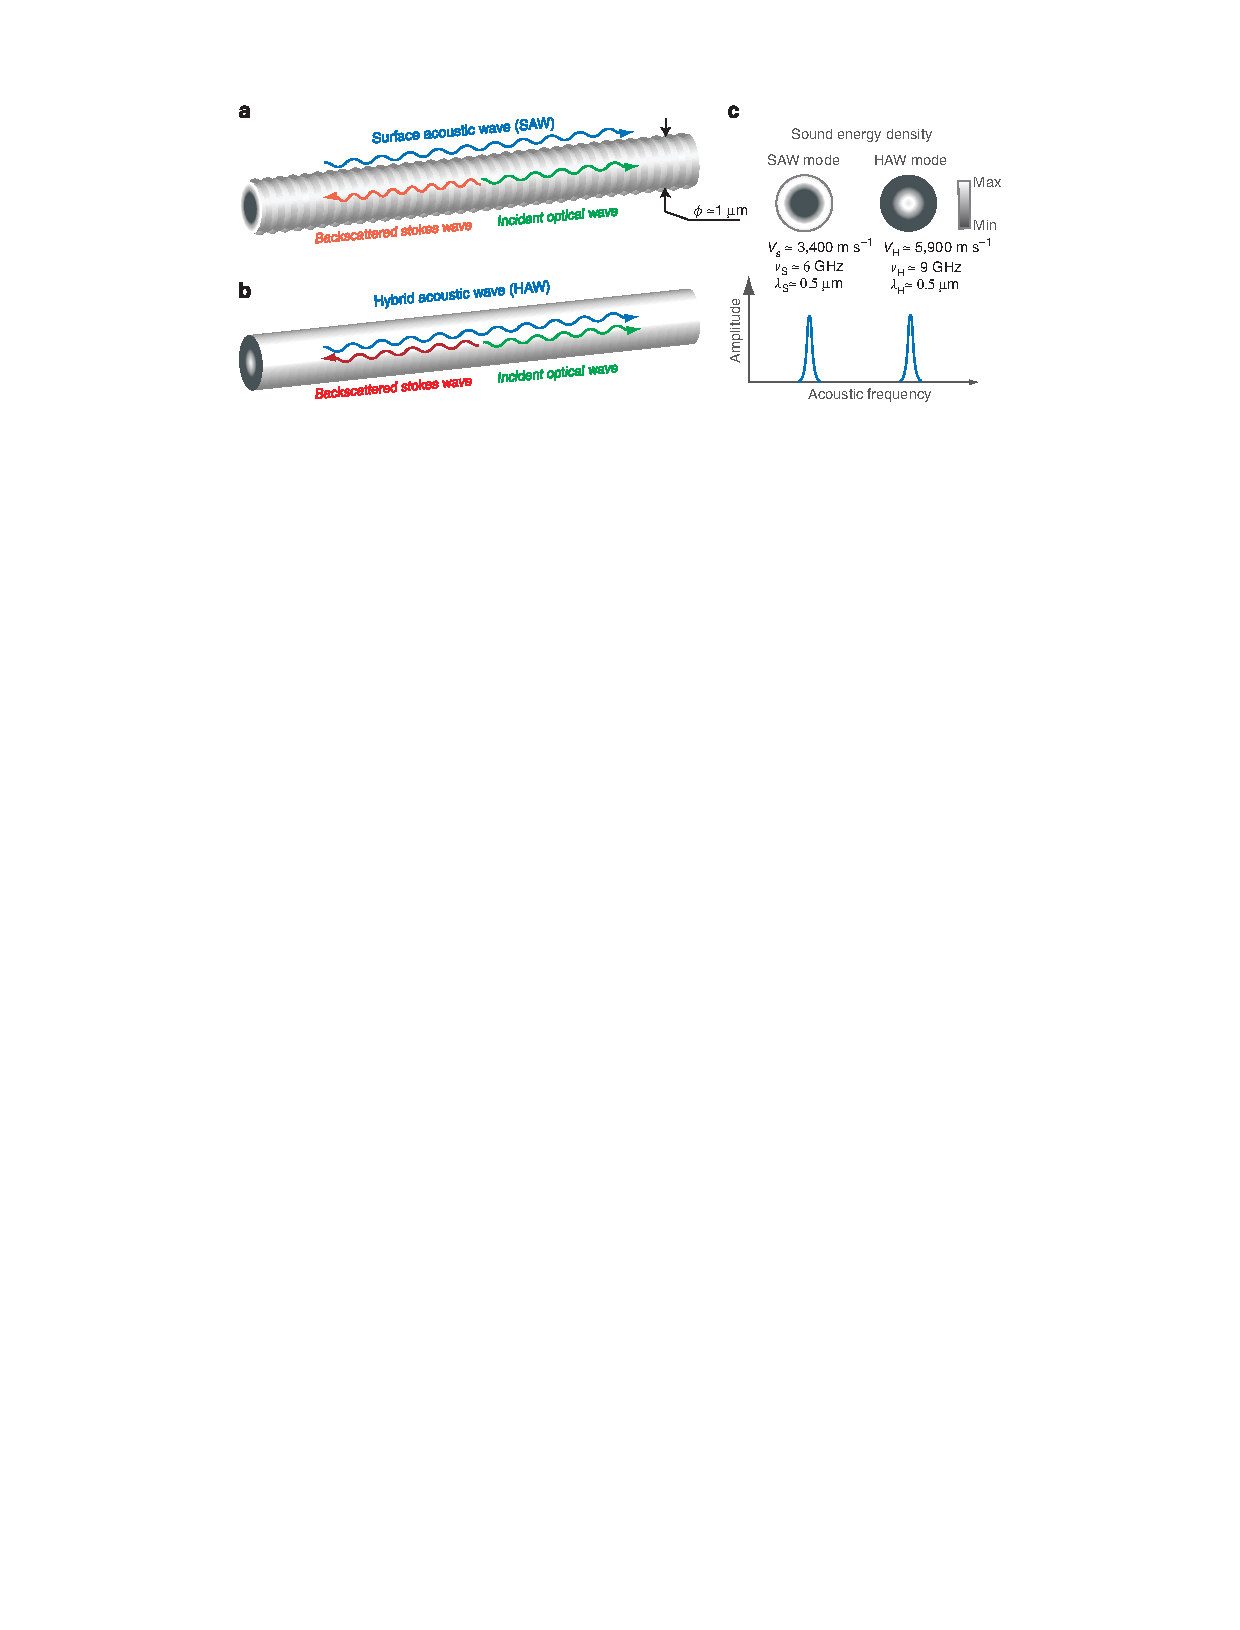
\includegraphics[width=1.0\columnwidth]{f1.pdf}
\end{center}
\end{frame}

%%%%%%%%%%%%%%%%%%%%%%%%%%%%%%%%%%%%%

\begin{frame}
\frametitle{Experimental implementation}
\begin{center}
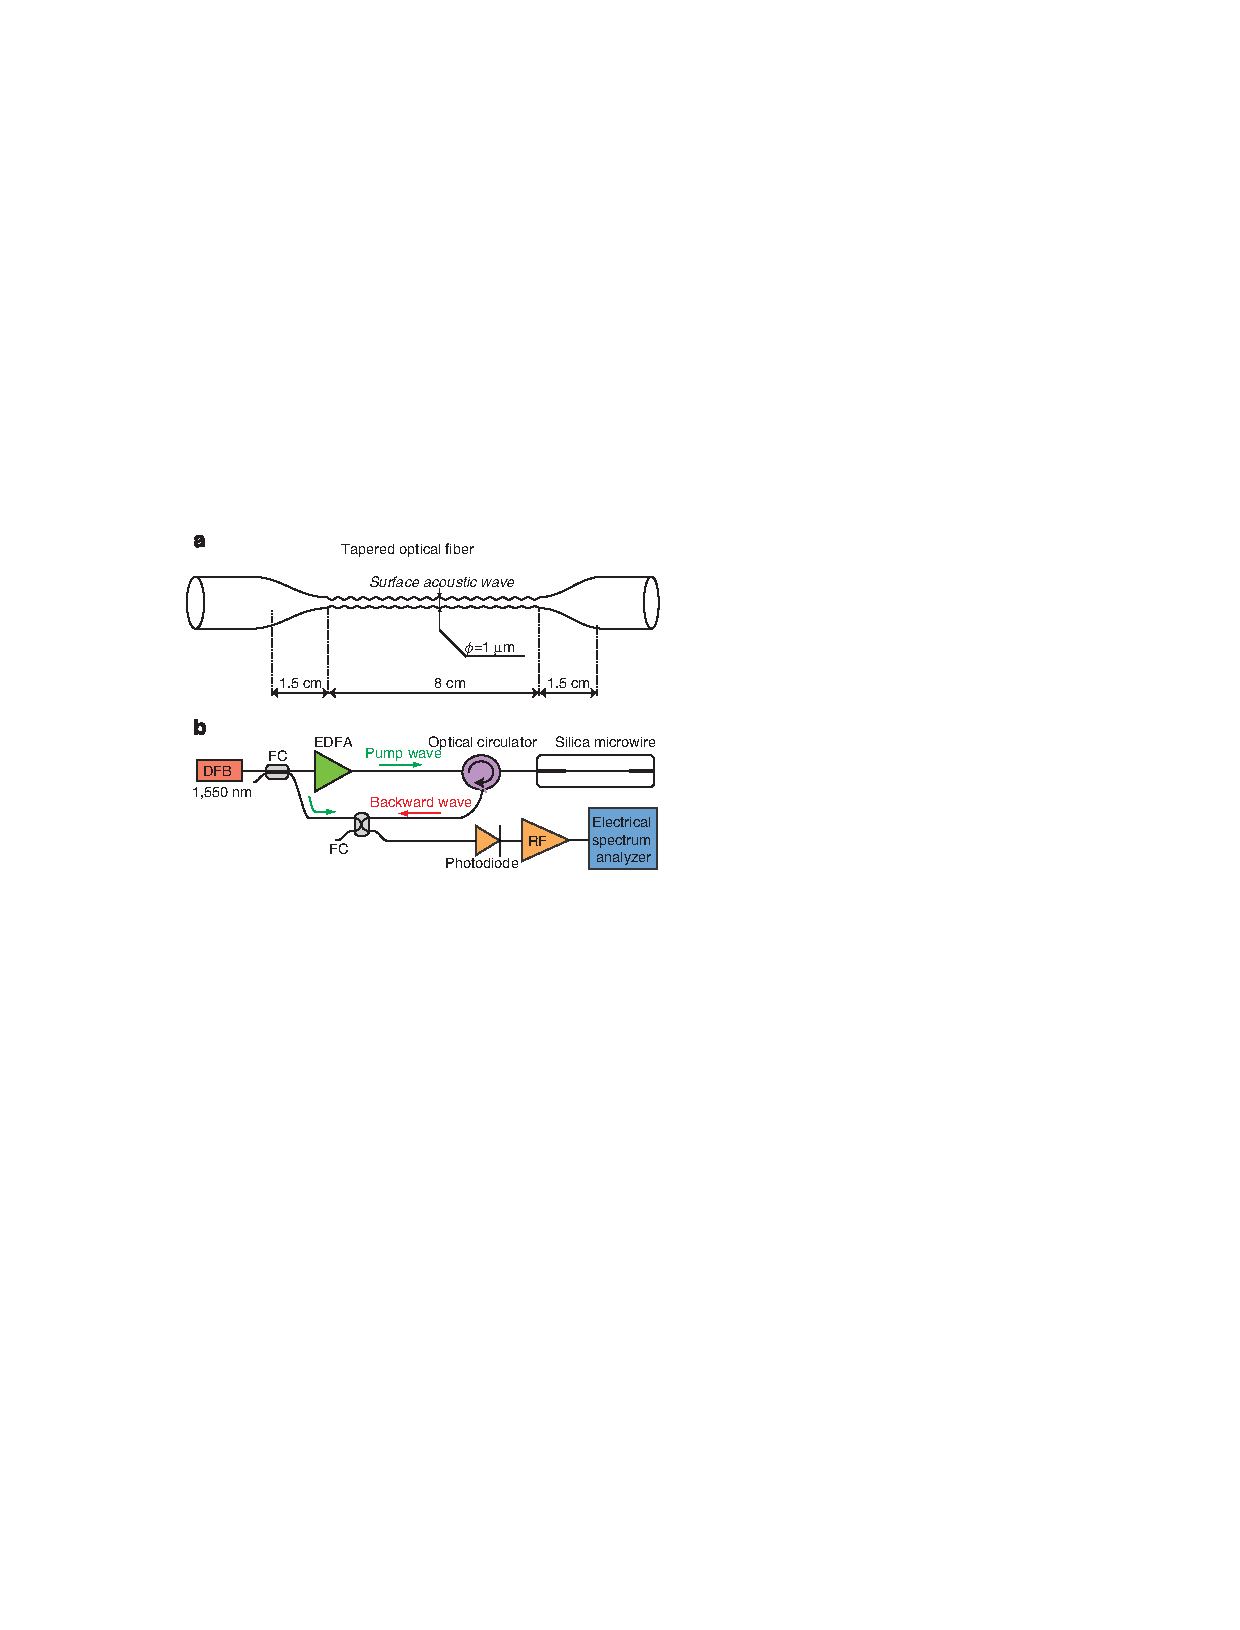
\includegraphics[width=0.8\columnwidth]{f2ab.pdf}
\end{center}
\end{frame}

\begin{frame}
\frametitle{Results and simulation}
\begin{center}
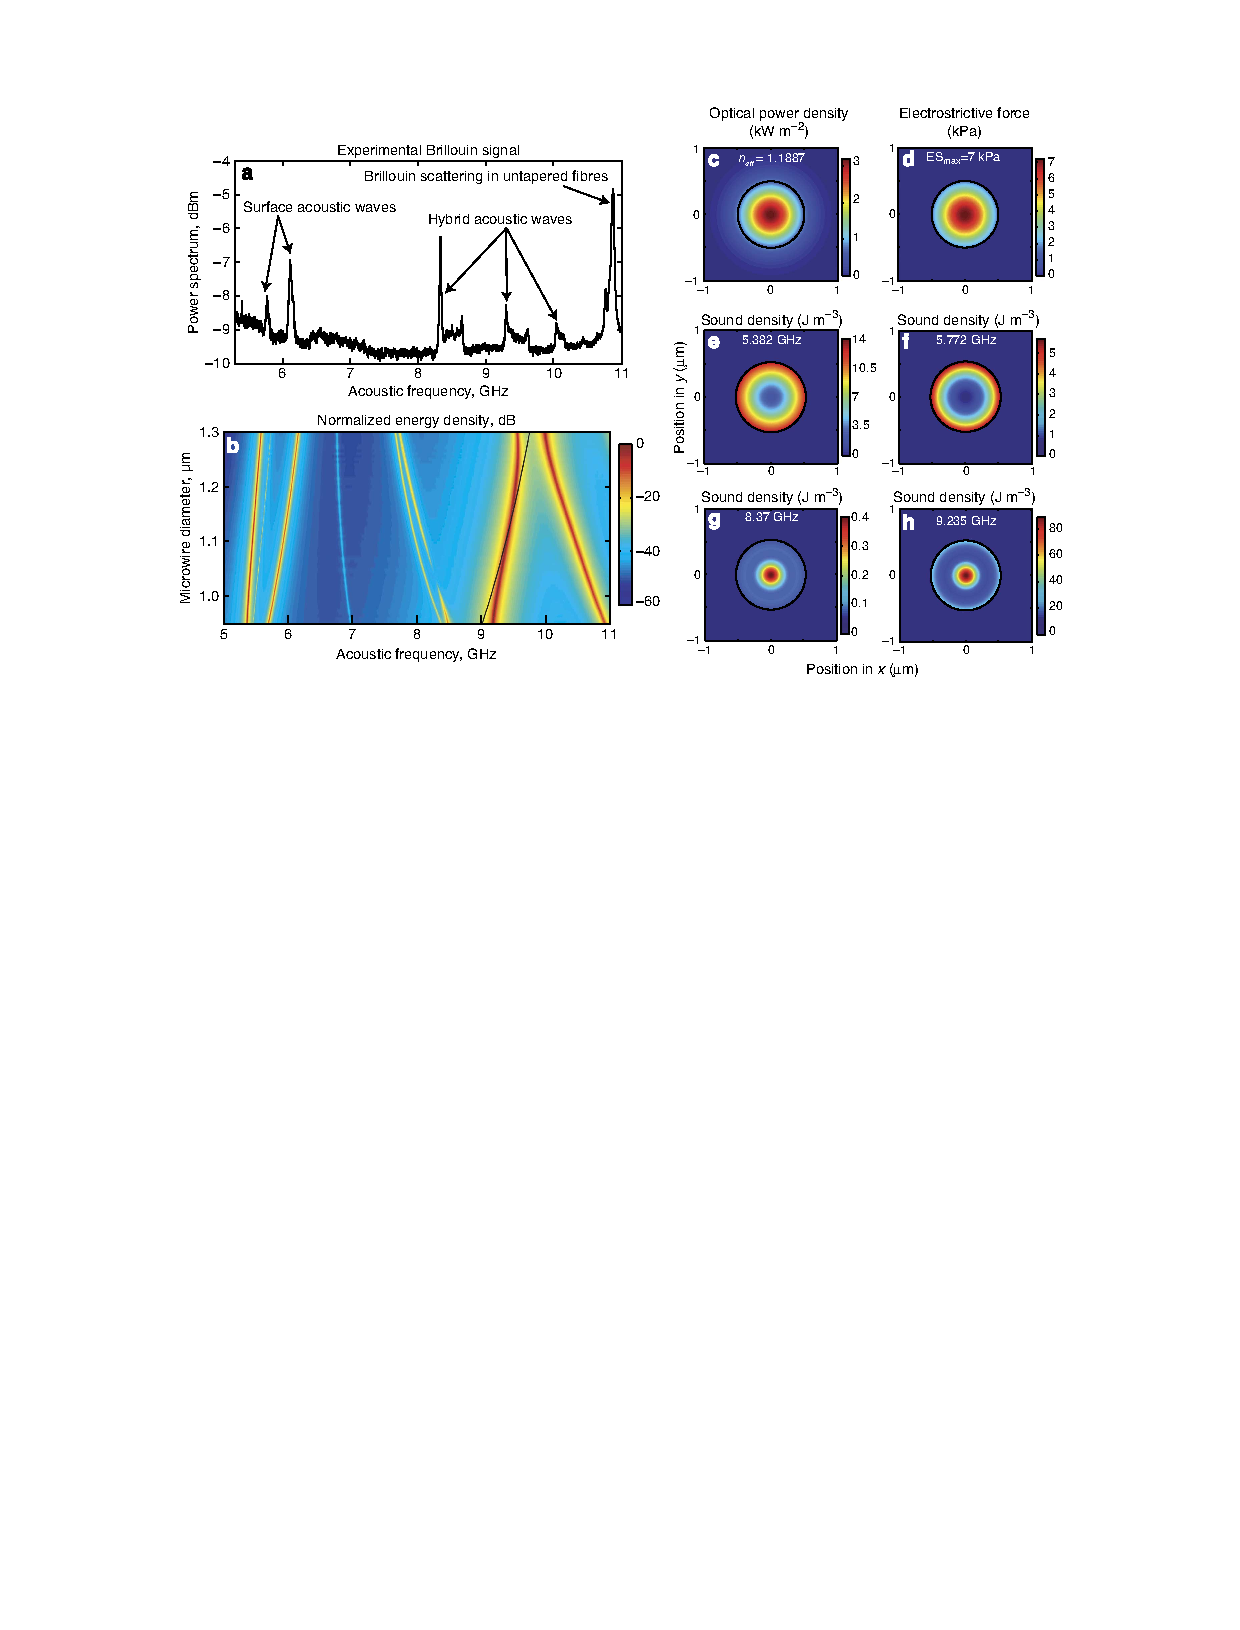
\includegraphics[width=1.0\columnwidth]{f3.pdf}
\end{center}
\end{frame}

\begin{frame}
\frametitle{Numerical simulations of the full acoustic wave spectrum}
\begin{center}
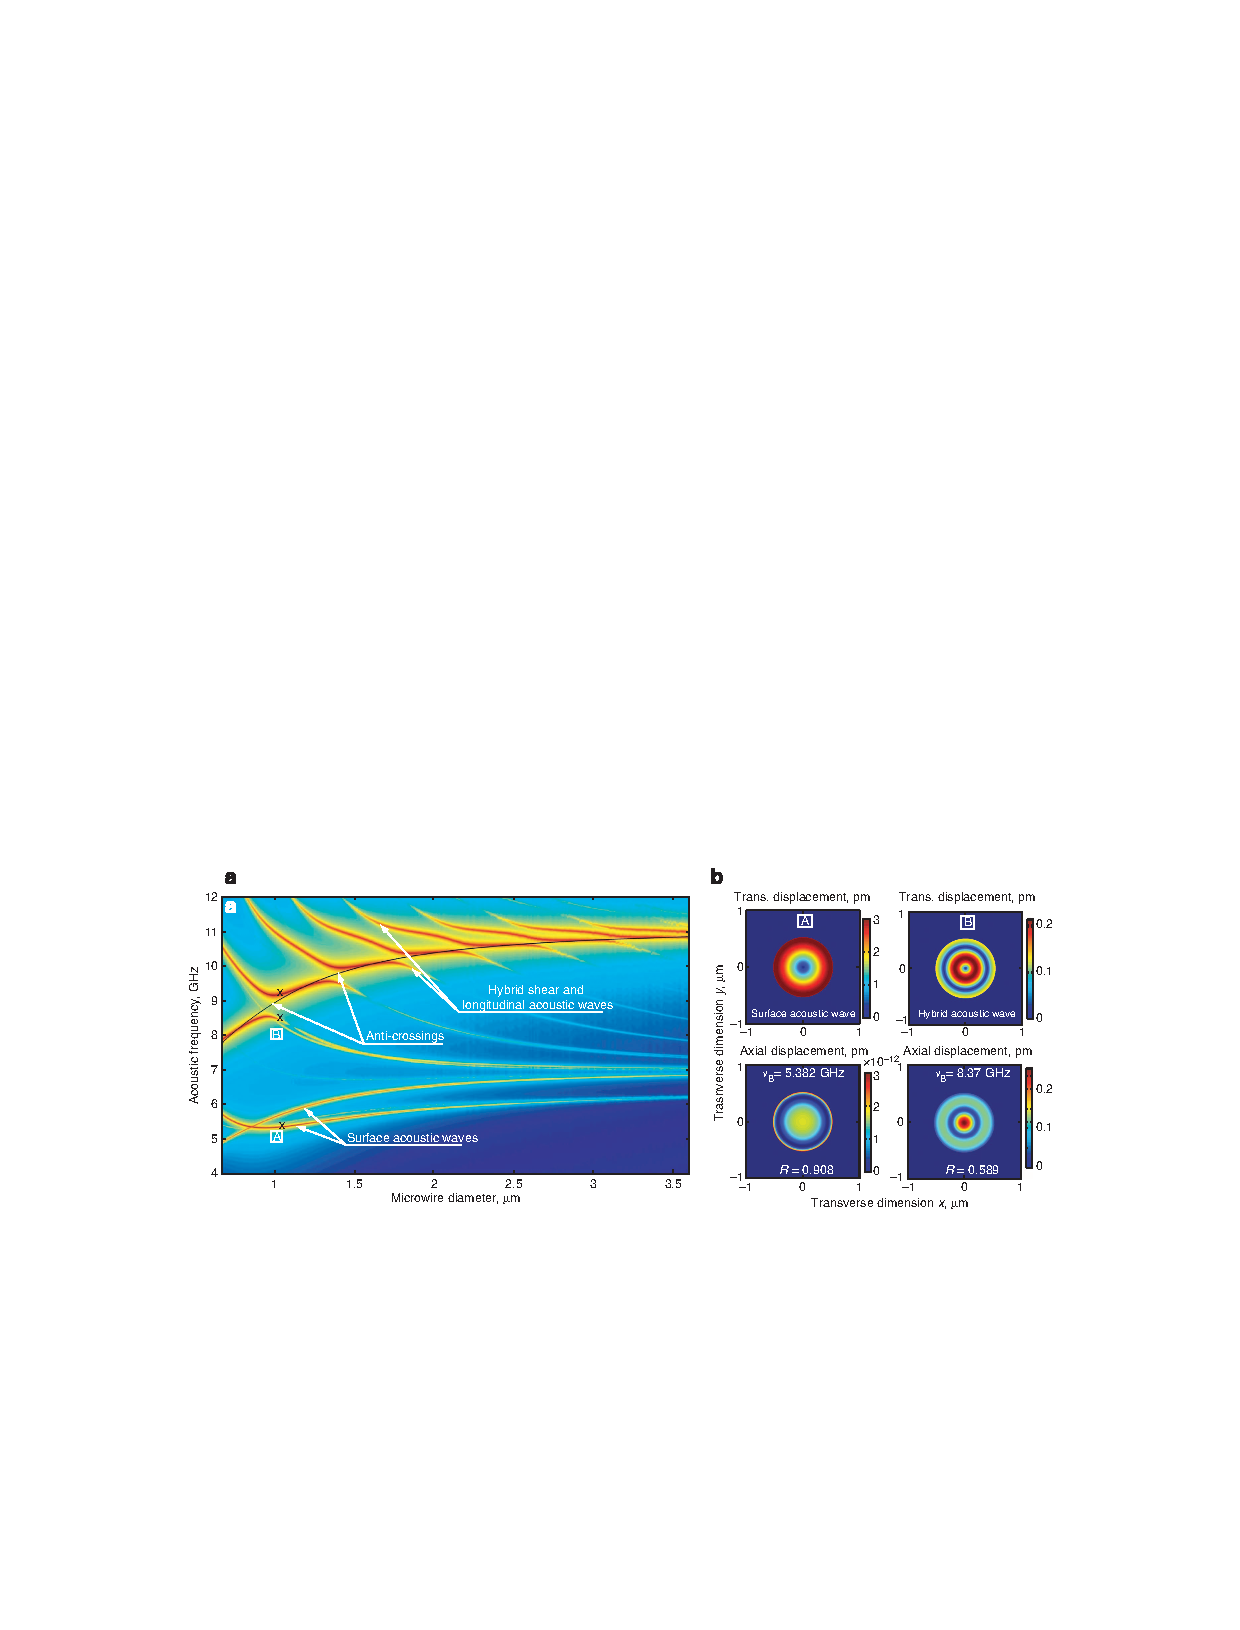
\includegraphics[width=1.0\columnwidth]{f4.pdf}
\end{center}
\end{frame}

\begin{frame}
\frametitle{Brillouin gain and threshold for the stimulated regime}

Brillouin gain:
\begin{equation*}
g_B = \frac{4\pi n_{\mathrm{eff}}^8P_{12}^2}{c\rho\lambda^3\nu_B\Delta\nu_B}
\end{equation*}

for SAW in subwavelegth fiber:
\begin{equation*}
\begin{aligned}
g_B &= 1.4\times 10^{-12}\,\mathrm{mW}^{-1}\\
\frac{g_B}{A_{\mathrm{eff}}} &= 8\, \mathrm{W}^{-1}\mathrm{m}^{-1}
\end{aligned}
\end{equation*}

for HAW in  fiber:
\begin{equation*}
\begin{aligned}
g_B &= 3\times 10^{-11}\,\mathrm{mW}^{-1}\\
\frac{g_B}{A_{\mathrm{eff}}} &= 0.4\, \mathrm{W}^{-1}\mathrm{m}^{-1}
\end{aligned}
\end{equation*}


Threshold:
\begin{equation*}
P_{\mathrm{th}}=\frac{21A_{\mathrm{eff}}}{Kg_BL_{\mathrm{eff}}}
\end{equation*}
\end{frame}

%%%%%%%%%%%%%%%%%%%%%%%%%%%%%%%%%%%%

\begin{frame}
\frametitle{More on Brillouin scattering}
\framesubtitle{Stimulated optomechanical excitation of SAW}
\begin{center}
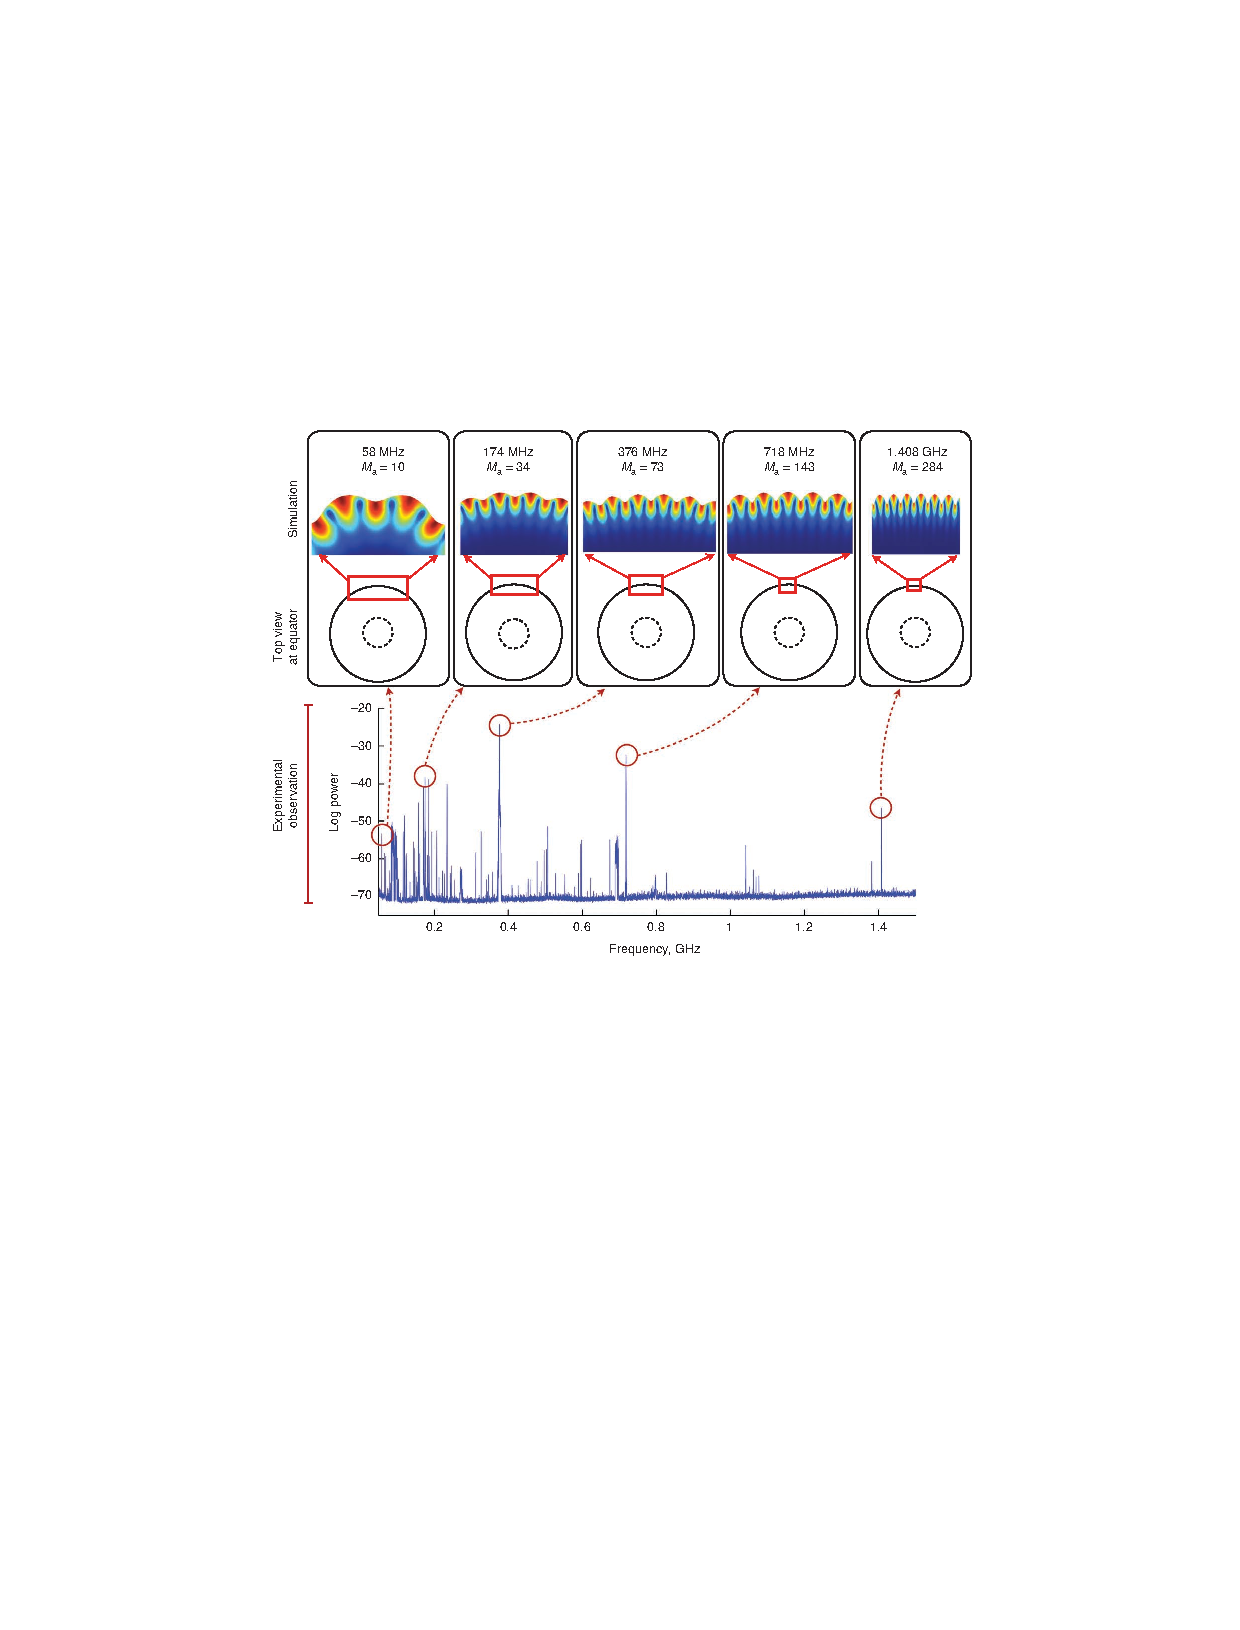
\includegraphics[width=0.8\columnwidth]{f5.pdf}
\end{center}


\noindent\rule{0.1\textwidth}{0.5pt}

\begin{itemize}
\item \tiny{Bahl, G. \etal Nat. Commun \textbf{2}, 403 (2011).
}
\end{itemize}
\end{frame}

%%%%%%%%%%%%%%%%%%%%%%%%%%%%%%%%%%

\begin{frame}
\frametitle{More on Brillouin scattering}
\framesubtitle{Observation of spontaneous Brillouin cooling}

\vspace{4em}

\begin{columns}[onlytextwidth]
\begin{column}{0.6\textwidth}
\begin{center}
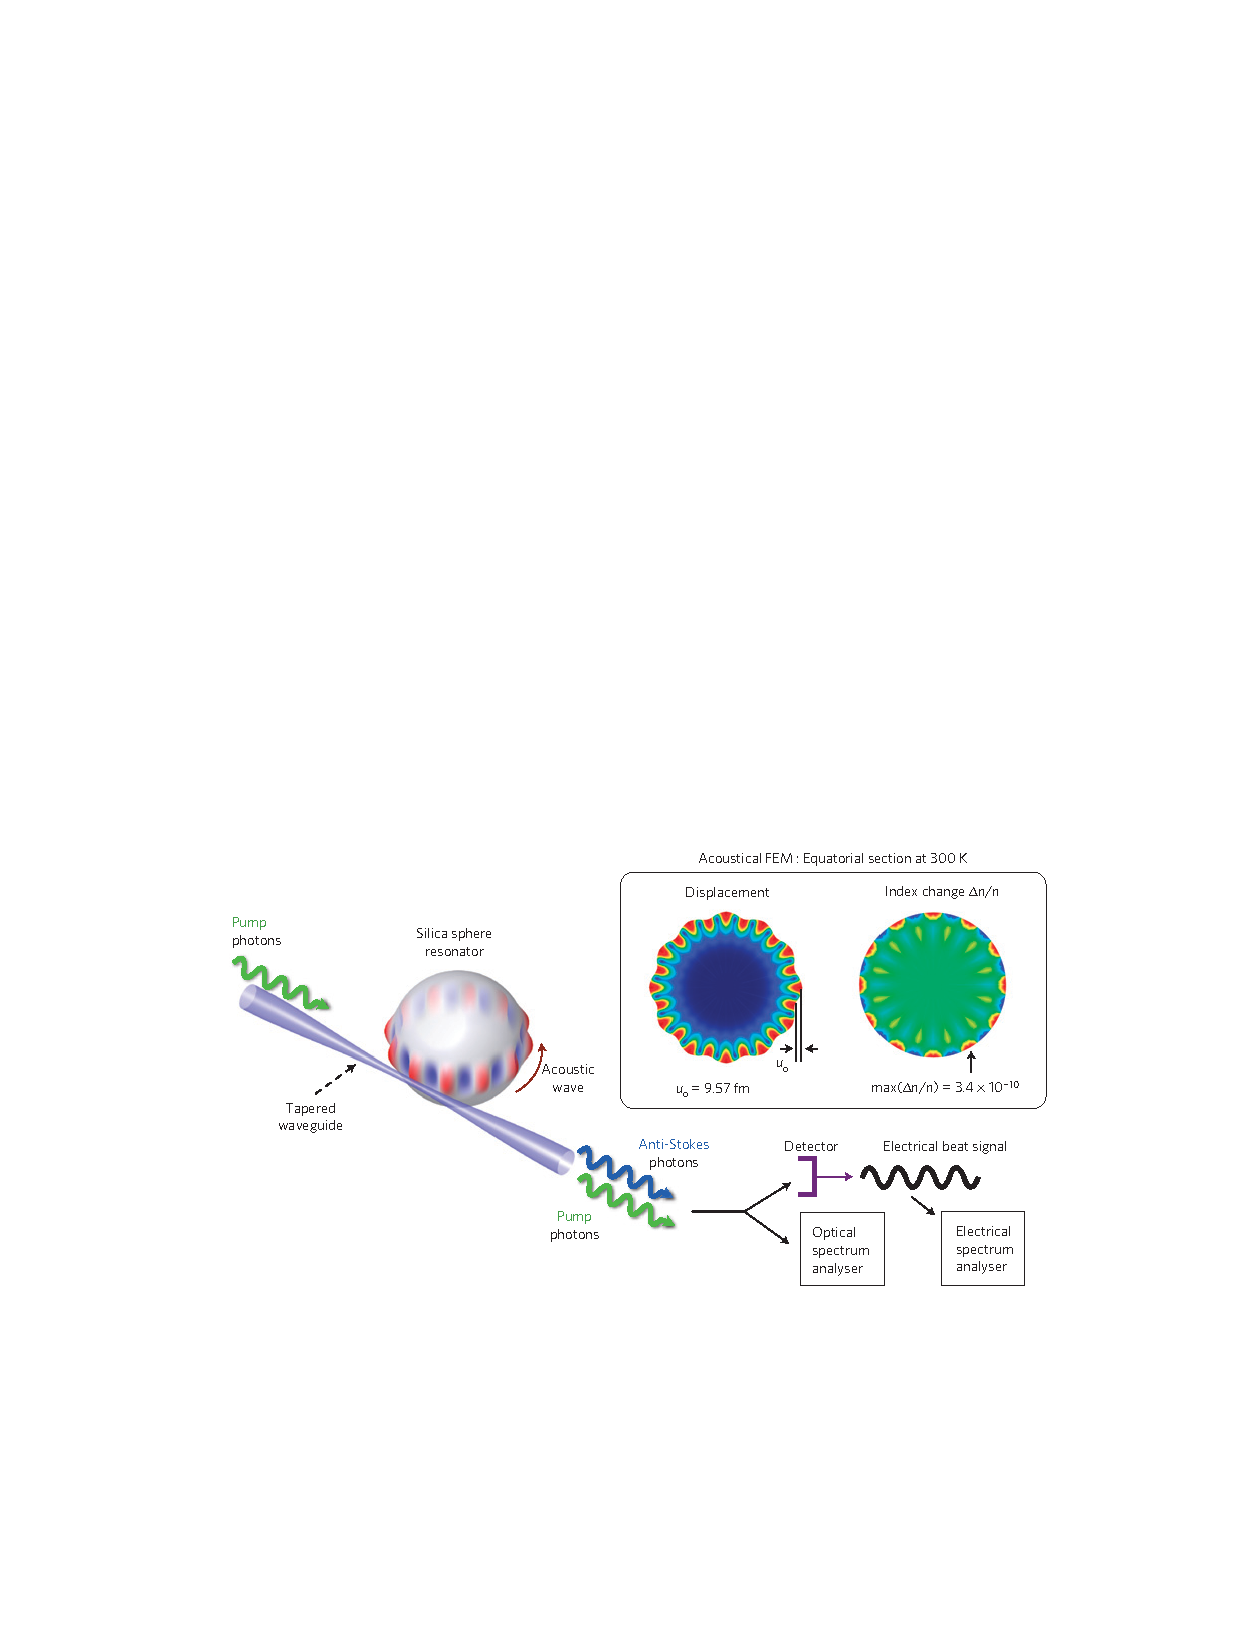
\includegraphics[width=1.0\columnwidth]{f6.pdf}
\end{center}
\end{column}
\begin{column}{0.4\textwidth}
\begin{center}
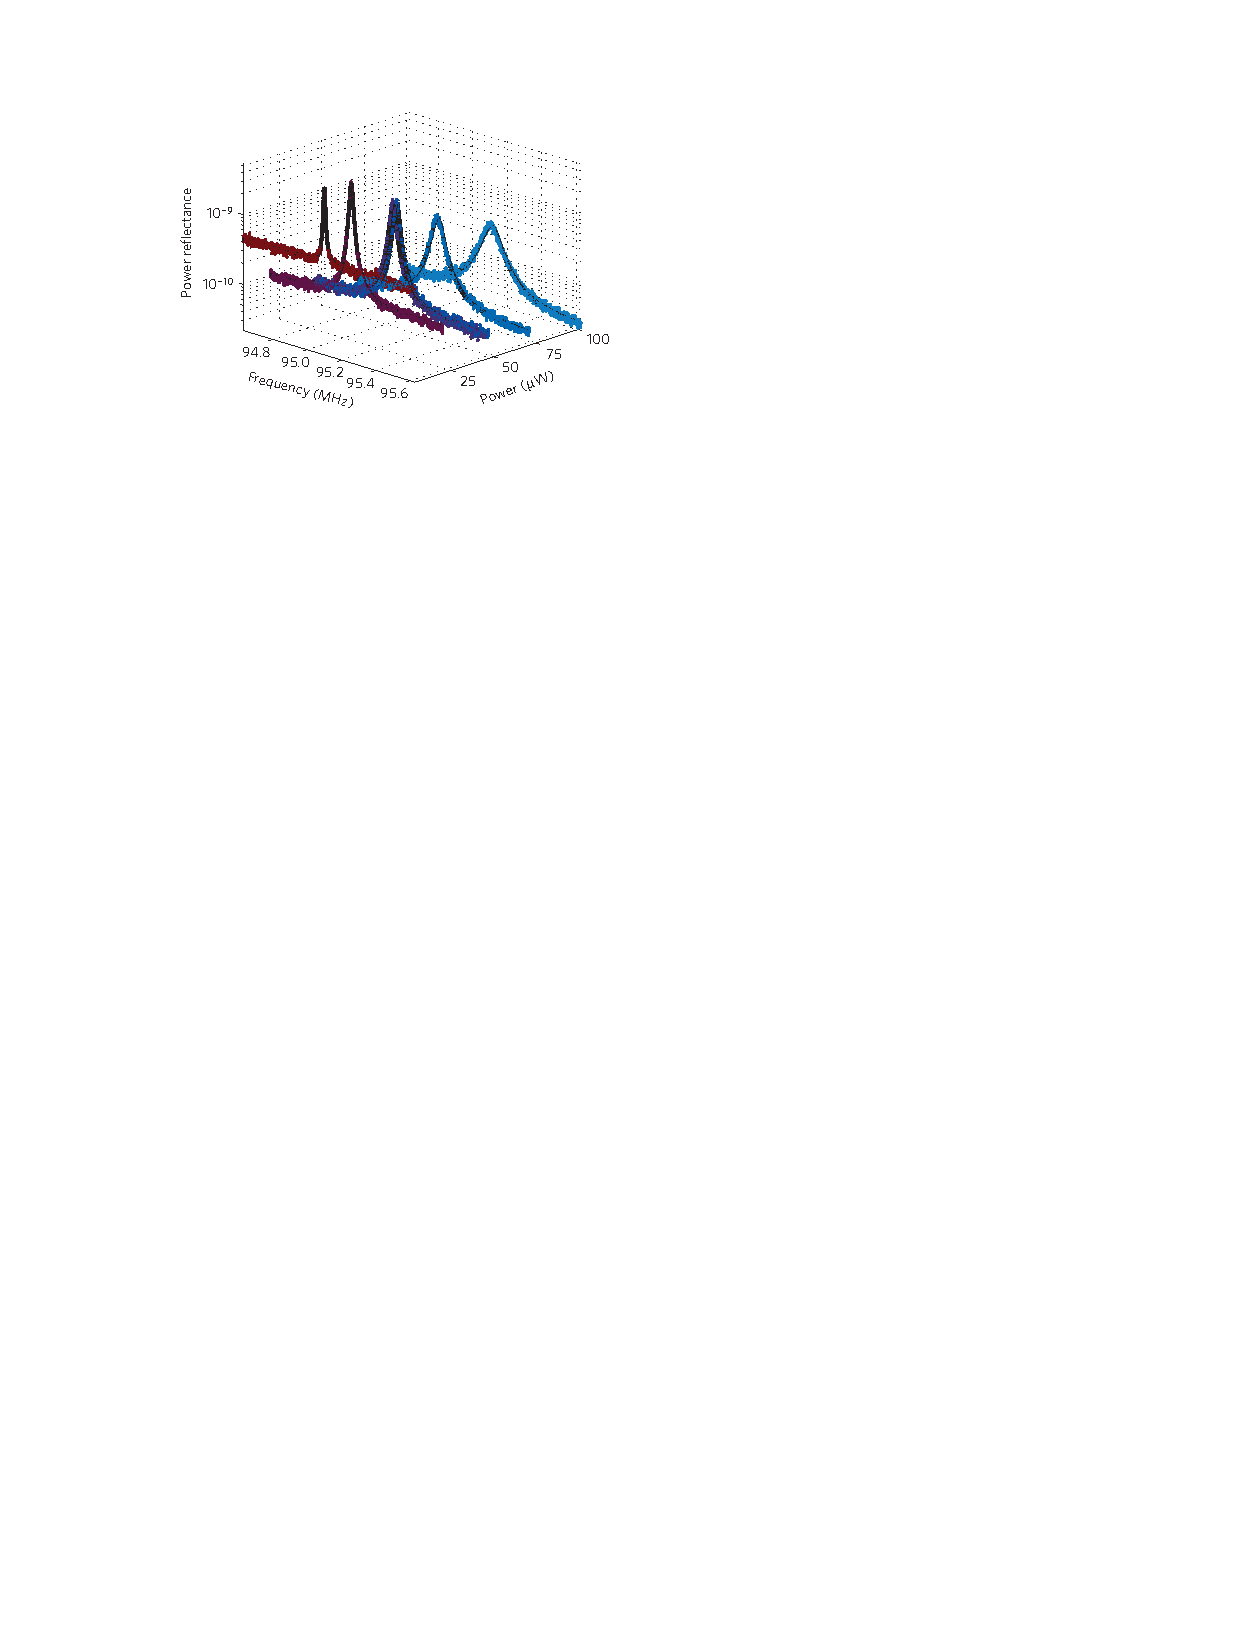
\includegraphics[width=1.0\columnwidth]{f7.pdf}
\end{center}
\end{column}
\end{columns}

\vspace{4em}
\noindent\rule{0.1\textwidth}{0.5pt}

\begin{itemize}
\item \tiny{Bahl, G. \etal Nat. Phys. \textbf{8}, 203–207 (2012).}
\end{itemize}
\end{frame}

%%%%%%%%%%%%%%%%%%%%%%%%%%%%%%%%%%%%%%%%%%%%%%%%%%%%%

\begin{frame}
\frametitle{More on Brillouin scattering}
\framesubtitle{Brillouin-scattering-induced transparency}
\vspace{3em}

\begin{center}
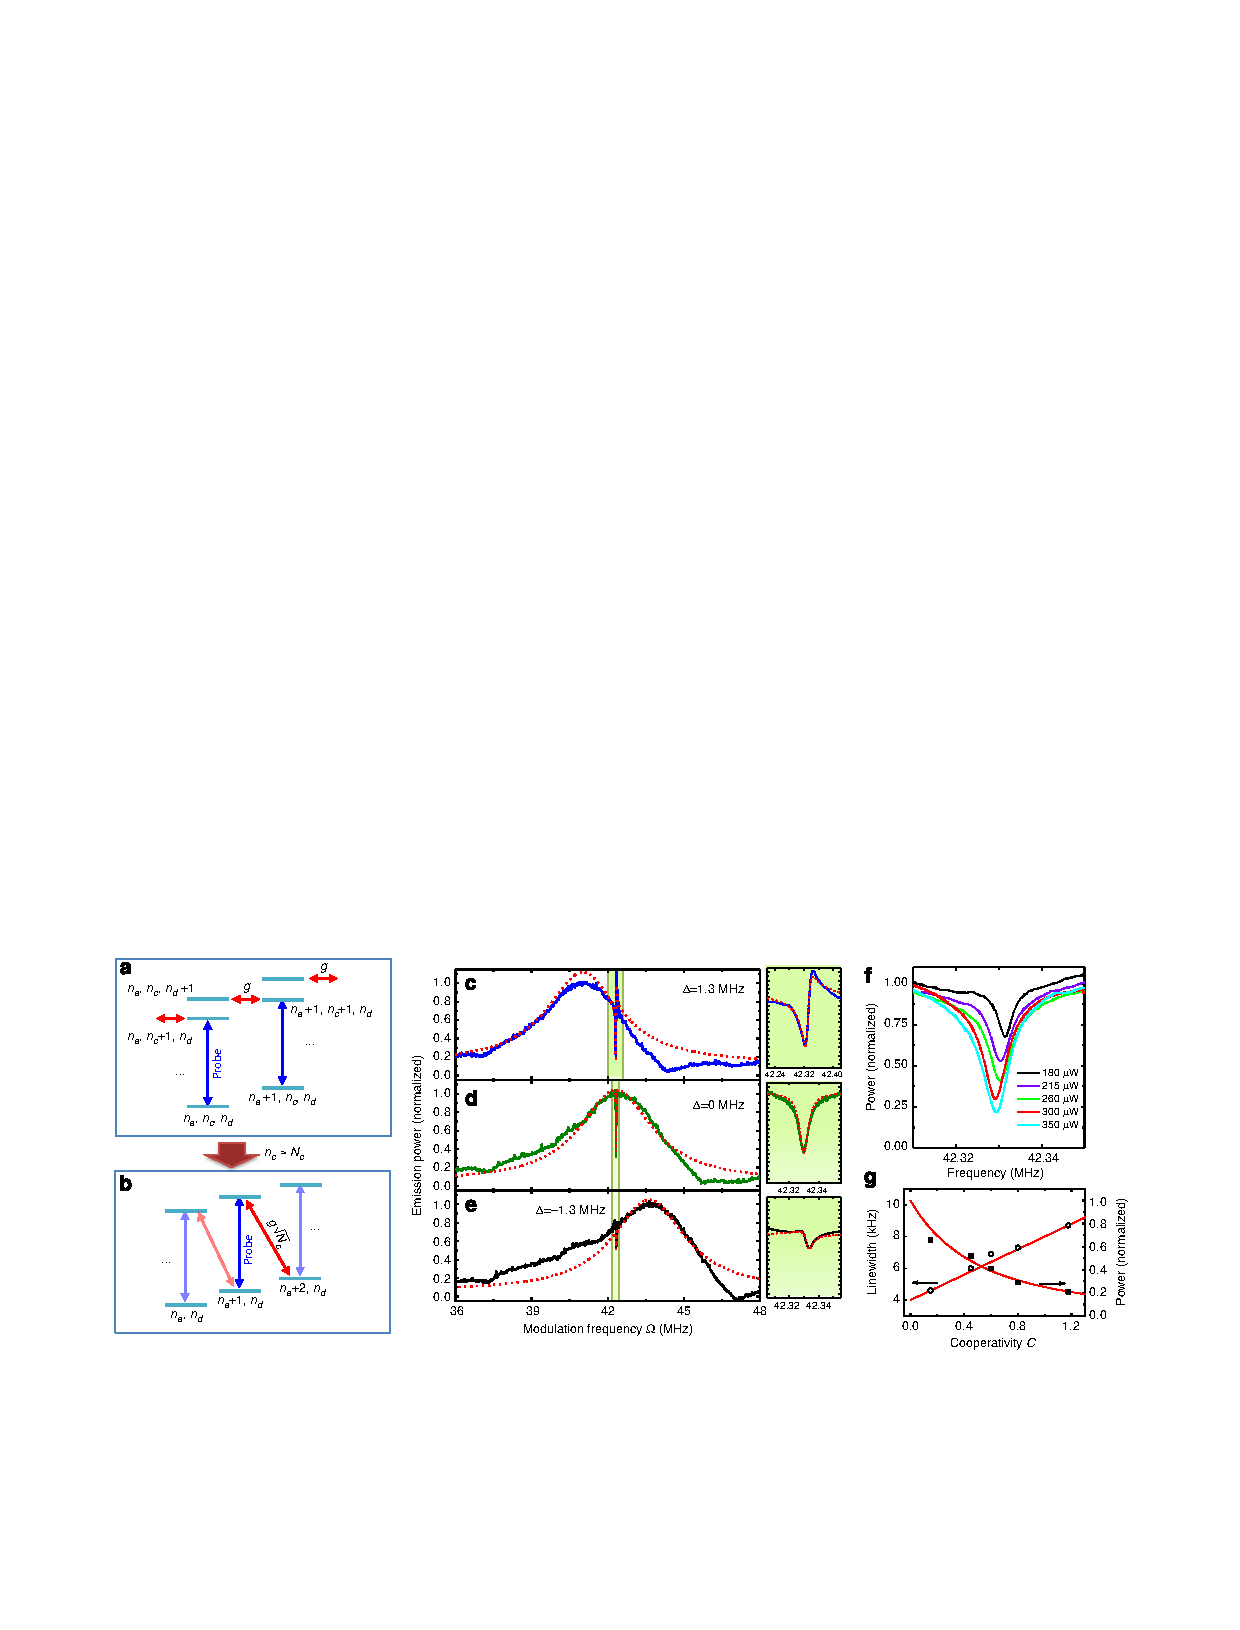
\includegraphics[width=1.0\columnwidth]{f8.pdf}
\end{center}

\vspace{3em}
\noindent\rule{0.1\textwidth}{0.5pt}

\begin{itemize}
\item \tiny{Dong, C.-H. \etal Nat. Commun \textbf{6}, 6193 (2015).

}
\end{itemize}
\end{frame}

%%%%%%%%%%%%%%%%%%%%%%%%%%%%%%%%%%%%%%%%%%%%%%%%%%%%%

% \begin{frame}
% \frametitle{More on Brillouin scattering}
% \framesubtitle{Non-reciprocal light storage}
%
%
% \begin{center}
% 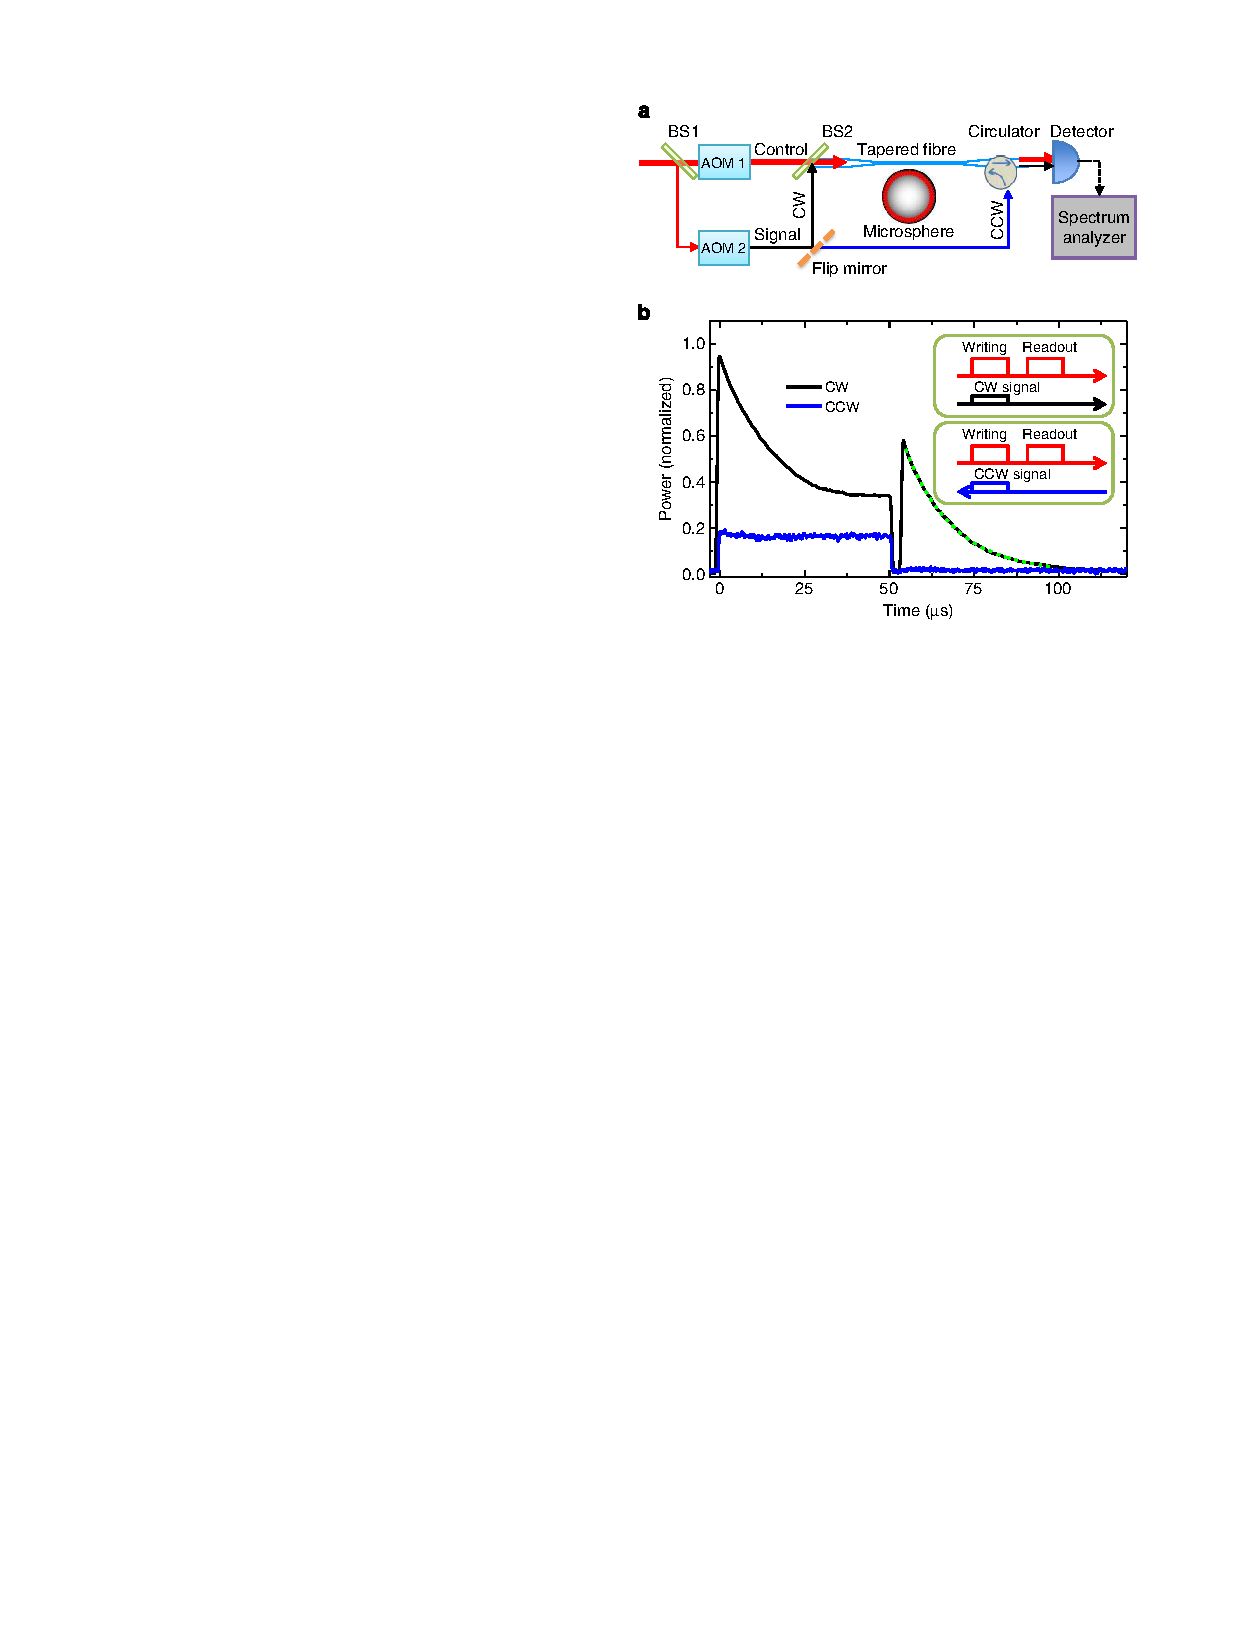
\includegraphics[width=0.6\columnwidth]{f9.pdf}
% \end{center}
%
%
% \noindent\rule{0.1\textwidth}{0.5pt}
%
% \begin{itemize}
% \item \tiny{Dong, C.-H. \etal Nat. Commun \textbf{6}, 6193 (2015).
%
% }
% \end{itemize}
% \end{frame}



\end{document}
